\documentclass{acm_proc_article-sp}
\usepackage{times}
\usepackage{url}
\usepackage{changepage}
\usepackage{latexsym}
\usepackage{amssymb}
\setcounter{tocdepth}{3}
\usepackage{graphicx}
\usepackage{CJKutf8}
\usepackage{mdwlist}
%\usepackage{indentfirst}
%\usepackage{amsmath,amsthm,amssymb}
\newtheorem{definition}{Definition}
\newtheorem{hypothesis}{hypothesis}
\newtheorem{theorem}{Theorem}
\setlength\parindent{0pt}

\usepackage{color}
\newcommand{\mo}[1]{\textcolor{red}{#1}}

%\newtheorem{theorem}{Theorem}
%\setlength\titlebox{6.5cm}    % You can expand the title box if you
% really have to
\begin{document}
\title{Resonation Elicits Diffusion: Modeling Subjectivity of Users and Tweets for Retweeting Analysis}

\maketitle
%\mo{retweet is a text and retweeting is an action. Most "retweet" in this paper need replace by "retweeting".}
\begin{abstract}
Retweet is the core mechanism of information diffusion on Twitter, and many factors have been proved to influence retweet behavior, however few studies have investigated the subjective aspect of a user to retweet a message. Subjective nature of human is the underlying motivation of diverse social behaviors including information diffusion, and subjective resonation triggered by topic and opinion similarity between tweets and users will elicit retweeting behaviors.
%\mo{(The motivation is too weak!!)}
In this paper, in the light of psychological theory, we put forward that a tweet is more likely to be retweeted by a user because of similar subjectivity, and propose a subjective model to combine both the topics and opinions to model subjectivity of users and tweets. Technically, We use the state-of-the-art Latent Dirichlet Allocation topic model to find the topics users are talking about, and sentiment analysis techniques to determine user's opinions towards these topics from user-generated content simultaneously. 
We evaluate our model in the retweet analysis problem to verify its influence on retweet behavior and effectiveness in the retweet prediction performance. \mo{(you should  give more details about ur approach and experimental result)}
\end{abstract}

% A category with the (minimum) three required fields
\category{H.4}{Information Systems Applications}{Miscellaneous}
%A category including the fourth, optional field follows...
\category{H.3.3}{Information Search and Retrieval}{Information filtering}[performance measures]

\terms{Model, Experimentation}

\keywords{Twitter, subjectivity, retweet, LDA, sentiment analysis} % NOT required for Proceedings

\section{Introduction}
\label{introduction}
Twitter is well-known for its freedom of publishing short message (i.e. tweet) within a limited length of 140 characters, and viral spreading of information across complex social networks.
Since launched in March 2006, the service rapidly has gained worldwide popularity, with over 500 million registered users at the end of year 2012, who generated over 340 million tweets per day\footnote{\url{http://en.wikipedia.org/wiki/Twitter}}.
In addition to large amounts of user-generated content, Twitter provides its social network functions for connection, communication and information diffusion by allowing users to message one another directly and follow one another publicly. 
The complex networks and large content volume of Twitter provide researchers with insights into people’s social behavior on a scale that has never been possible \cite{DBLP:conf/hicss/StieglitzD12}.

Information diffusion is a lasting research for social scientists who might want to study the problem on Twitter because an established convention of Twitter facilitates information diffusion \mo{(I can not understand this 	
sentence)}. 
Despite the restricted length of tweets, retweet convention and complex networks of Twitter provide an unprecedented mechanism for the spread of information \cite{Jenders:2013APV}. 
Actually almost a quarter of the tweets published by users are retweeted from others \cite{conf/cikm/YangGCTLZS10}. 
Therefore, it is important to understand how retweet works which can help study information diffusion on Twitter. 


Although several studies on retweeting have concentrated on analyzing retweet habits and influencing factors \cite{Boyd2010,Kwak:2010TSN,Suh2010}, most of them are generic, not user oriented.
From the point of a user, retweet is a process that includes reading the tweet, estimating the worth of content and deciding to share. The crucial part of this process is estimating the worth that a message containing information interested to the user.
%From the point of a user, the process of retweeting includes reading the tweet, deciding whether it is worthwhile to share and acting on it, hence retweet behavior indicates that the user considers the tweet containing information interesting to him.
Therefore modeling the interest of users provides an important perspective for retweet behavior analysis. 
%In this study we focus specifically on how information spreads on Twitter by exploring underlying reasons that a user retweets a particular tweet out of the overwhelming message flow 
In this study we focus specifically on how information spreads on Twitter by exploring the retweet behaviors of users.
\mo{(moved this sentence into this passage which gives the motivation of your work.)}. 

Previous studies on the retweet behaviors of users have shown that an enriched user model gives coherent and consistent explanation for retweet behavior \cite{Abel:2011AUM,conf/icwsm/MacskassyM11,conf/wsdm/FengW13}  \mo{(I can not understand this 	
sentence)}. Specifically, researchers have tried to model users from four types of information:
profile features ("\textbf{Who you are}"), tweeting behavior ("\textbf{How you tweet}"), linguistic content ("\textbf{What you tweet}") and social network ("\textbf{Who you tweet}") \cite{Pennacchiotti:icwsm11}. 
Despite demographic profile, tweeting habits and network connections might determine source and scope of information users could be exposed to, topics of interest of users encapsulated in rich linguistic content have been proved consistently valuable for retweet behavior explanation \cite{conf/icwsm/MacskassyM11}. Moreover,
Petrovic \emph{et al.}~\cite{Osborne_Lavrenko_2011} and Hong \emph{et al.}~\cite{ericmedvet:hong2011} found whether a tweet will be propagated is largely about identifying the topics of interest \mo{(Here you should give a text and citation of previous work about the topic affecting retweet. \textbf{By the way, if the citation is the part of a sentence, you must cite the paper as my way, please change all the citations!!!})}. However, beyond merely news and events (related to the topic), Twitter has become a platform where large amounts of opinions are presented and exchanged by the users. Existing research demonstrated that user-generated content with rich sentiment information can trigger more attention, feedback or participation \cite{DBLP:conf/hicss/StieglitzD12}, and tweets with high emotional diversity have a better chance of being retweeted \cite{conf/icwsm/PfitznerGS12}. Therefore, although users consume thousands of tweets about different topics every day, the tweet whether will be retweeted might depends on the subjective choice of users. 

Philosophically, subjective initiative nature of human determines that the pattern of behavior is subjectivity driven.
Psychological researchers have identified subjectivity as the underlying factor that influence the decision-making about taking what activities to process incoming stimul \cite{Moore2008}.
According to theory of Biased Assimilation, bias is an inherent feature of human subjectivity, and bias is a consistent, robust characteristic of behavior, so people are prone to choose and diffuse information according to their own biased subjectivity \cite{Hyman2000,sunstein2009rumors}.
It can be inferred from above explanation that users are prone to diffuse a tweet that can raise resonation with their biased subjectivities. \mo{(I suggest you could delete all preceding text and merge this passage into the preceding passage.)} Intuitively, subjectivity can be represented as topics and opinions articulated in the information generated by users on Twitter.  In this study we explore the textual information of Twitter to model the subjectivity of tweets and users, and investigate whether the subjective model could benefit the retweet behavior analysis. 


Modeling subjectivity of tweets and users on Twitter is a challenge study as the sparsity of textual information, the changes of topics and opinions over time,  informal language, etc.
However, we are interested in understanding retweet behavior at a local level rather than at a global level, since most of time retweet behavior pertains to a local network of the tweet publisher and followers. As a result the relatively tiny size of local network and topic homophily lower the impact of sparsity.
Given the biased nature of subjectivity, while new information may arise and old information may change their meaning, biased subjectivity to be more consistent and less prone to external perturbations, unless users actually change their interests and opinions, which is usually a relatively long process.

\mo{(Delete it!!! You should change the following text into the approach and your experiment in detail.)}
Our work aims to define and establish the subjective model and identify the role of subjectivity in the processes of information diffusion on Twitter.
By using ``\textbf{Subjectivity}'' , we refer to both topics of users' interests and users' opinions towards these topics, so we model users not only by topics they care about, but also by ``\textbf{what they think about the topics}''. 

\mo{(Contributions is too weak. You should show your idea and task, your novel approach, your exciting experimental result)} Our contributions can be summarized as follows:
\begin{itemize*}
\item Based on psychological theory, we put forward formal definition of subjective model for users and tweets.
\item Based on state-of-the-art topic model and sentiment analysis technique, we propose the method of establishing subjective 
model from user-generated content on Twitter.
\item Combined with the retweet behavior analysis problem, we analyze the impact of subjective model on retweet behavior and compare our model with other modeling methods.
\end{itemize*}
The rest of the paper is organized as follows: section 2 gives related work to our research, the proposed subjective model is defined and specified in section 3, the qualitative and quantitative evaluation is described in section 4. Section 5 summarizes the paper and points to future work.

\section{Related Work \mo{please change all the citations!!!}}
\label{relatedwork}
In this section, we give an introduction to three lines of relevant research work: $ 1) $ retweet behavior analysis, $ 2) $ user profile and user modeling, and $  3)$ sentiment analysis. 
\subsection{Retweet behavior analysis}
A large body of studies have analyzed characteristics of retweet, examining factors that lead to increased retweetability and designing models to estimate the probability of being retweeted. 

As for factors influencing retweetability, \cite{Suh2010} found that tweets with URLs and hashtags were more likely to be retweeted, and there was a strong linear relationship between the number of followers and the likelihood that the tweet be retweeted. 
\cite{conf/icwsm/MacskassyM11} studied a set of Twitter users over a period of a month and sought to explain the individual retweet behaviors.
They found that models derived from tweets content could explain most of retweet behaviors.
\cite{Comarela:2012UFA} found previous response to the tweeter, the tweeters’ sending rate, the freshness of information, the length of tweet could affect followers’ response to retweet. 
\cite{Starbird:2012RRI} addressed specifically the retweet mechanism during crises. 
They found that tweets with topical keywords were more likely to be retweeted. 

There were also work extending the analysis to build retweet prediction model. 
\cite{conf/cikm/YangGCTLZS10} designed features from factors that influence the retweet behavior and built a semi-supervised framework on a factor graph model to predict users’ retweet behaviors. 
\cite{Osborne_Lavrenko_2011} introduced features such as novelty of a tweet and the number of times the author is listed to train a model with a passive aggressive algorithm. 
They found the dominance of social features, while tweet features added a substantial boost to the performance.
\cite{Jenders:2013APV} analyzed the "obvious" and "latent" features from structural, content-based, and sentimental aspects of both tweet and users, with respect to their impact on the spread of tweets. 
They found a combination of features covering all aspects was the key to high prediction quality.
\cite{Naveed:2011SMC,2011:NaveedGKC} introduced interestingness as static quality measure to capture the static content quality of tweets, and quantified it based on such features as emoticons, sentiments and topics a tweet contains, then trained a logistic regression model to predict the probability of retweet for an individual tweet .
\cite{conf/wsdm/FengW13} built a graph made up of users, publishers and tweets nodes with all sources of information incorporating into nodes and edges, and proposed a feature-aware factorization model to re-rank the tweets according to their probability of being retweeted.
\cite{conf/icwsm/PfitznerGS12} proposed a new measure called emotional divergence to evaluate the retweet probability of a tweet and showed that highly emotional diverse tweets can have up to almost five times higher chances of being retweeted.

From a global perspective, all papers introduced above tried to answer the question of ``Which tweets will be retweeted by anyone or not?''. 
But they are weak to capture ``Whether a tweet is retweetable from a user-centric perspective considering the interests and opinions of users''. 
In this paper, we will try to answer this question by building a subjective model which can capture both the interests and opinions of users.

\subsection{User profile and user modeling}
With the popularity of social media, researchers have begun to pay close attention to the massive amount of data generated by users, and put forwards several techniques to model users on the data. These studies provide researchers with insights into user online behaviors. 

\cite{Hannon:2010} proposed that Twitter users can be modeled by the tweets and the relation of Twitter social network.
They found that the approach based on social graph could explore users who are "near" in the sense of follow relations, but failed to find users who are "distant ", on the other hands, content-based approach could find similar users based on interests extracted from the content of tweets. 
\cite{conf/icwsm/MacskassyM11} discover user's topics of interest by leveraging Wikipedia as external knowledge to determine a common set of high-level categories that covers entities in tweets. 
\cite{RamageEtAl:10} made use of topic models to analyze Twitter content at large scale and at the level of individual users with 4S dimensions, showing improved performance on tasks such as post filtering and user recommendation. 
These efforts about user modeling on Twitter have simply built model for each user by extracting keywords, entities, categories or latent topics from tweet content. 

Some researchers argued that user behavior could easily be affected by some external factors other than user interest.
\cite{Xu:2012MUP} proposed a mixture model which incorporated three important factors, namely breaking news, friends' time-line and user interest, to explain user posting behavior.
\cite{Pennacchiotti:icwsm11} proposed the most comprehensive method to model Twitter user for user classification. They focused on richer feature sets such as features derived from topic models, tweet sentiment analysis and explicit follower-followed links, to exploit the user-created content. 
Their work confirmed the value of in-depth features which reflect a deeper understanding of the Twitter user and the user network structure.

As introduced in Section~\ref{introduction}, previous researches have tried to model users from four types of information: profile features, tweeting behavior, linguistic content and social network. 
Some studies perceive that the implicit features articulated in the user-generated content play an important role in user behavior analysis,  and they have proposed diverse techniques to capture such in-depth features to model user's interest. 
Additionally, a few of work identifies the correlation between sentiment of users and their behaviors.
But they all fail to model subjectivity of a user as a whole.
Motivated by the observation, we firstly put forward subjective model to combine both interests and opinions to model a holistic user. \mo{Tense Error}

\subsection{Sentiment Analysis}
Sentiment analysis is a popular research area for many years. Previous research mainly focused on reviews or news comments. 
%Generally, there are two major methods: rule-based approach and machine learning approach. 
Recently, the research began to pay more and more attention in social media such as Twitter
% because of the massive user-generated content and the unique characteristics which could be incorporated into sentiment analysis. 
 
\cite{Hu:2013www} interpreted emotional signals available in social media data for unsupervised sentiment analysis by providing a unified way to model two main categories of emotional signals: emotion indication and emotion correlation. 
\cite{Jiang:2011TTS} focused on target-dependent Twitter sentiment classification, they proposed a method to improve target-dependent Twitter sentiment classification by taking target-dependent features and related tweets into consideration. 
\cite{AsiaeeT:2012} presented a cascaded classifier framework for per-tweet sentiment analysis by extracting tweets about a desired target subject, separating tweets with sentiment, and setting apart positive from negative tweets.
\cite{Hu:2013ESR} extracted sentiment relations between tweets based on social theories, and proposed a novel sociological approach to utilize sentiment relations between messages to facilitate sentiment classification and effectively handle noisy Twitter data.
Motivated by sociological theories that humans tend to have consistently biased opinions, \cite{CalaisGuerra:2011BOT} addressed challenges of topic-based real-time sentiment analysis by proposing a novel transfer learning approach with a suitable source task of opinion holder bias prediction.
\cite{Thelwall:2010SSS,Thelwall:2012SSD} designed SentiStrength, an algorithm for extracting sentiment strength from informal English text with human-evaluated dictionaries for words connotated with positive or negative sentiment strength, which exploited the grammar and spelling styles in typical microblogs.
In this paper, we adopt SentiStrength for sentiment analysis to build our subjective model, as a finer grain sentiment strength could give us more detailed opinion of users than binary polarized sentiment.

\section{Subjective Model (\mo{This section should rewrite!!!}).}
\label{subjectivemodel}
In this section, we firstly give the definition of subjective model. Then we describe the method of building subjective model. Finally, we formulate the retweet analysis problem with subjective model(\mo{It is strange to use "formulate"}).
\subsection{Definition}
\label{definition}
%Psychologically, the subjectivity of human is the underlying reason that drives his social behavior (\mo{Here gives citation.}). When a user browses a tweet in the message flow, the inner subjectivity determine his choice of retweeting, which depends on whether the topics and the opinions of the tweet could resonate with the user. If the topics and opinions of a tweet are familiar with the user's interest and attitude, the user is likely to propagate it.  (\mo{The last two sentences have the same meaning, you could delete one of them}). The core problem lies in that how to model the subjectivity of the user and the tweet (we refer subjectivity of tweet as the topics it talks about and the opinions towards these topics it holds  (\mo{You could put this sentence into abstract.})). 

Subjectivity has been studied extensively by psychologists from different dimensions. These  dimensions include characterizing the personality of people based on such records as historic behaviors and remarks \cite{Engbert2007}, and linguists have defined the subjectivity of language as the speaker always shows their perspectives, attitudes and sentiments in the discourse \cite{stein2005subjectivity}.  (\mo{I can not understand}). 
The user-generated content of social media provide massive language data that traditional collection methods can not achieve.
Using these data, we firstly give our definition of subjective model on Twitter. Here we emphasize that our model can be used in other social media platforms as well. \mo{Saying the reason that you model the tweet and user.}. 

\mo{Here you'd better give the definition of $U$, $T$, $O$, etc}. 

\begin{definition}[Subjective Model For User]
The subjective model of a user $\mathrm{u \in U}$ is a set of topics $\mathrm{t_{i} \left( i \in \lbrace1 \cdots n \rbrace \right) }$ 
the user talks about in a topic space $\mathrm{T}$ and the user's opinions $\mathrm{o_{i}}$ towards these topics. \mo{No text of motivation for this definition; Is a model a set of topic and opinions? Or topics and opinionsdistribution?}. 
\begin{equation}
\label{usermodel}
P \left( u \right) = \lbrace \left( t_{i}, w_{u} \left( t_{i} \right), d_{u,t_{i}} \left( o_{i} \right) \right) \,\vert  t_{i} \in T, \, o_{i} \in O \rbrace
\end{equation}
where:
\begin{itemize*}
\item with respect to the given user $\mathrm{u}$,  for each topic $\mathrm{t_{i} \in T}$, its  weight $\mathrm{ w_{u} \left( t_{i} \right)}$ represents the distribution of the user's interests on it.
\item opinion $\mathrm{o_{i}}$ of user towards topic $\mathrm{t_{i}}$ is a target-dependent sentiment distribution  $\mathrm{d_{u,t_{i}} \left( o_{i} \right)}$ over sentiment valence space $O$.
\end{itemize*}
\end{definition}

As medium for the users to express themselves, tweets are also subjective to some extent (\mo{I can not understand this sentence and you'd better give the motivation of modeling the tweet}). In order to calculate the similarity of subjectivity between a  tweet and a user, the subjective model of a tweet is given as follows:

\begin{definition}[Subjective Model For Tweet] \mo{There is the same problem as before.}. 
The subjective model of a tweet $\mathrm{c \in C}$ is a set of topics $\mathrm{t_{i} \left( i \in \lbrace1 \cdots n \rbrace \right) }$ it talks about in the same topic space $\mathrm{T}$ as the users, and the opinions $\mathrm{o_{i}}$ it expresses towards these topics.
\begin{equation}
\label{tweetmodel}
P \left( c \right) = \lbrace \left( t_{i}, w_{c} \left( t_{i} \right), d_{c,t_{i}} \left( o_{i} \right) \right) \,\vert  t_{i} \in T, \, o_{i} \in O \rbrace
\end{equation}
\end{definition}

\subsection{Retweet Problem Statement}
\label{statement}
Although subjective model might explain several behaviors of social media users, we are interested in retweet behavior in this paper, and apply subjective model to understanding underlying mechanism of information diffusion at a micro-level. \mo{Delete the preceding text. You should say retweet is very important user behavior on Twitter, therefore we investigate whether our subjective model can help understand this process.} 
It has been demonstrated that any retweeted tweet is able to reach an average of 1,000 users no matter how many followers the publisher of original tweet has \cite{Kwak:2010TSN}. \mo{Why did you say this?} 
Retweet function has given every user the power of spreading information broadly, and individual user has the power to dictate which information is important and should spread by pushing retweet button. \mo{Why did you say this?} 
In fact a user only retweets a small number of tweets and only small subset of followers actually retweet a tweet because the likelihood of a tweet to be retweeted depends on both network context and tweet content. 
Apart from network context, a tweet is more likely to be retweeted by users are who are interested in the tweet, therefore, we are not only interested in modeling the tweet by itself but also how the tweet resonates with the individuals who might decide to pass it on, and we put a much stronger emphasis on the content and try to model the user's retweeting decision by deriving high-level content-based topic and opinion features. \mo{I do not understand the whole paragraph.} 

In fact whether a tweet will be retweeted depends heavily on context such as the author's position in the social graph or the time of day the tweet is published. 
A tweet with only few or passive followers is less likely to be retweeted, and tweets published in the night have less chance to get retweeted than daytime. 
Despite such a fact, neither contextual factor has any influence on the content of a tweet, therefore we deliberately ignore context information to avoid introducing contextual bias into our analysis of retweet by proposing a hypothesis. 
\begin{hypothesis}[H1]
\label{hypothesis1}
A tweet is evenly visible to the followers who subscribe to it by following its publisher.
\end{hypothesis}
The rationale behind this hypothesis is, that the motivation of a user to retweet a tweet is that the user considers only the tweet content that arouse resonation with the user. \mo{I do not understand the whole paragraph either.} 

Studies have highlighted that Twitter network structure better resembles an information sharing network than an interconnecing social network \cite{Boyd2010,Kwak:2010TSN}. 
In the context of Twitter, the "following" relationship is a strong indicator of a phenomenon called "homophily", which has been observed in many social networks.
Homophily is a phenomenon that people of social network " are homogeneous with regard to many socio-demographic, behavioral, and intra-personal characteristics" \cite{mcpherson2001birds}.
In other words, homophily implies that a user follows another user because he is interested in what another user talks about in tweets, and another user follows back because he finds they share similar interests. 
According to the principle of homophily, we put forwards the concept of \textbf{Local Topic Space} that the content generated by users in the local network of a user and his followers concentrate on a few local topics.

If a tweet is published, all followers of publisher will receive it in their time-line. We suppose every follower will likely retweet it if he finds it worth to according to our hypothesis~\ref{hypothesis1}.
Ignoring the influence of context information, the goal of our study is understand whether the subjectivity of tweets and users can affect retweet.
% if so, the analysis of retweet will be reinforced by taking the subjective factor into account.
The problem we studied can be stated as follows:

Let $ F, P, C $ denote the follower set, publisher set and tweet set respectively. 
%As a tweet is created by only one publisher but can be received by multiple followers, 
A tweet $c$ ( $ c \in C $) can be defined as a tuple $ <f, p, c, r_{fpc}>  $ where: \mo{Delete $c$ in tuple?} 
\begin{itemize*}
\item  $p$ ($p \in P $) is the publisher of the tweet $c$ and $f$ ($ f \in F $) is a follower of publisher $p$.
\item $ r_{fpc} $ is a binary label indicating whether $ c $ is retweeted by $ f $.
\end{itemize*}

Our work focuses on using subjective model to analyze the relation between the subjectivity of a user and his retweet behavior. 
Hence we project \mo{(project?)} the tuple into the Local Topic Space $ T $, which is determined by the historic data of publisher $ p $ and followers $F $, and represent $ f, p, c $ with their subjective models established in $ T $ to analyze their relations with the retweet label $ r_{fpc} $ \mo{(I do not understand this sentence?)} .

\subsection{Retweet Problem Formulation With Subjective Model}
\label{concrete}
According to definition of subjective model, there are two distributions to model the subjectivity: one is topic distribution and the other is opinion distribution for each topic. Both of them are inferred from historic data produced by users.
As an open platform for collecting data, Twitter has become a valuable source for quantitative researchers in the last few years.
However, content analysis on Twitter has some challenges: the text of a tweet is very short with limit of 140 characters, informal languages are widely used which make many approaches based on supervised learning or natural language processing invalid. 
Hence modeling content on Twitter effectively requires techniques that can deal with this type of text .  \mo{ (little supervision needs gives the motivation of less training data)}.  \mo{Here, you should give a brief text of your techniques, such as LDA and SentiStrength.}
%In this section, we firstly proceed with detailed methods of how to establish subjective model, and then describe how to apply subjective model to the analysis of retweet behavior.
\subsubsection{Topic Analysis for Tweets}
\label{local}
As stated above, the relation of subjectivity between a publisher and a follower indicates their common interests in a Local Topic Space. 
%However, topics usually are not explicitly expressed by users, the topics of a tweet are latent features and have to be inferred by analyzing its content. The distillation of topics from tweet content requires methods that are suitable for short texts with heterogeneous vocabulary. 
The topics of a tweet are latent features and should be inferred from its content.
Although previous studies have tried to infer topics by finding keywords \cite{Chen:2010STE}, extracting  entities \cite{Abel:2011AUM} or linking tweets to external knowledge categories\cite{conf/icwsm/MacskassyM11},  topic model is still an effective way to modeling the topic of a tweet \mo{(give some citation about using topic model for tweets)}. Therefore we use \textbf{Latent Dirichlet Allocation (LDA)} to model the tweets and construct Local Topic Space for publisher and followers, since it is an efficient way to characterize latent topics in large corpus \cite{blei2003latent,conf/wsdm/WengLJH10}. 

%the sparsity is a main problem for these methods to model the users' interests because even users have common local topics they still might refer to a topic with different expressing way.
%Recent works show that topic models such as \textbf{Latent Dirichlet Allocation (LDA)} model and its extensions\cite{blei2003latent,conf/wsdm/WengLJH10} have been efficient ways to characterize latent topics of large volum corpus.  Topics of topic models are broader in concept than individual word, since a single topic consists of the whole collection of related words. Thus, the latent topics are more suitable to understand the common topics of interest among different users who use various words to describe the same topic. Therefore we use LDA model to find latent topics that are talked about between publisher and followers to construct their Local Topic Space. 

To distill the topics that users are interested in, documents of LDA should naturally correspond to tweets content. 
As our goal is to understand the topics that each user is interested in rather than the topics that each single tweet talks about, we aggregate the tweets published by each user into a single document. 
We adapt the original LDA model to the Twitter by replacing documents with aggregated tweet documents for every user in the local network\mo{(I do not understand this sentence.)}. 
Hence a user can be represented as a multinomial distribution over topics corresponding to the topic distribution of the user's subjective model.
The generative process can be graphically represented using plate notation in Figure~\ref{fig:graph2}. 

\begin{figure}[htb]
%\setlength{\belowcaptionskip}{-0.2cm} 
\centering
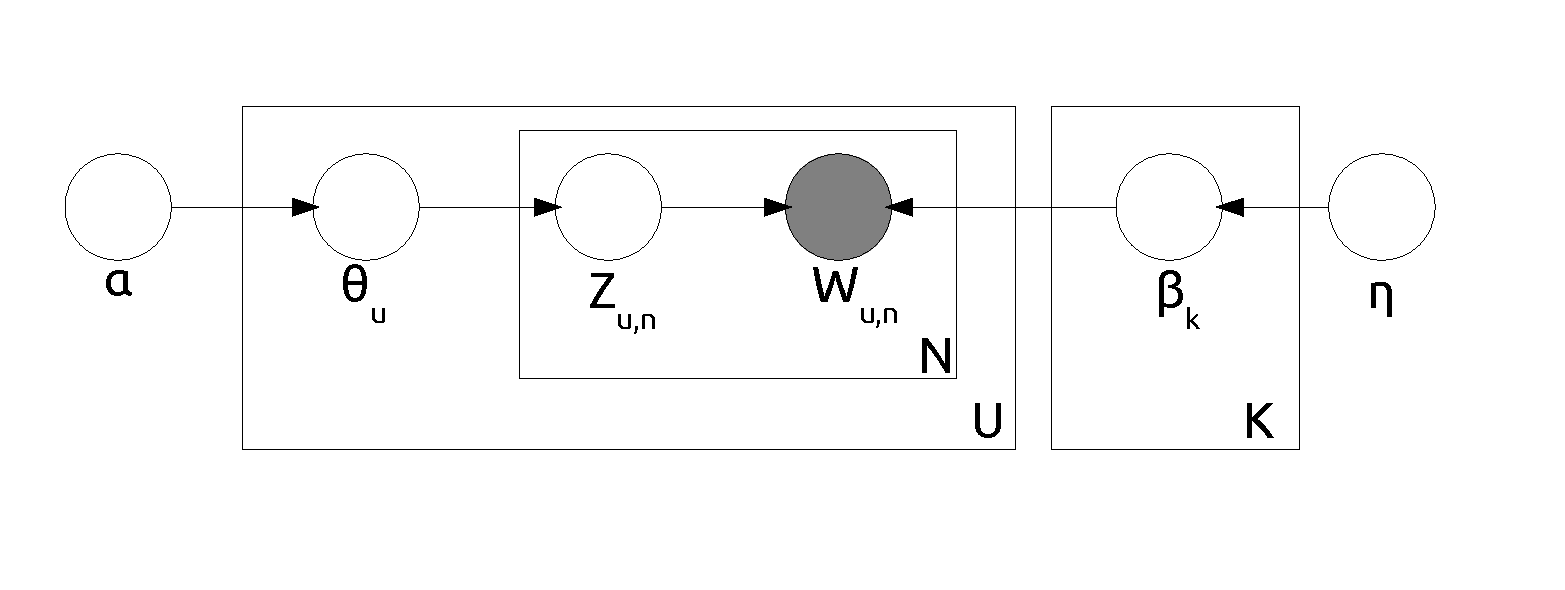
\includegraphics[width=3.0in,height=1.2in]{LDA.pdf}
%\vspace{-4em}
\caption{Plate illustration of the user-level LDA model.}
\label{fig:graph2}
\end{figure}

Formally, given a set of users $ U $ and the number of topics $ K $, a user $u$ ($ u \in U $) could be represented by a multinomial distribution $ \theta_{u} $ over topics with a Dirichlet prior parameterized by $ \alpha $. 
A topic $ k $ ($ k \in K $) is represented by a multinomial distribution $ \beta_{k} $ with another Dirichlet prior parameterized by $ \eta $. 
The generative process works as follows:
\begin{itemize*}
\item For each user $ u $, draw $ \theta_{u} \sim Dir \left(  \alpha \right) $.
\item For each word $ w_{u,n} $ in a user document, $ n \in \left\lbrace 1, \cdots, N \right\rbrace $ :
\begin{itemize*}
\item draw a topic $ z_{u,n} \sim Multinomial \left( \theta_{u}  \right) $;
\item draw a word $ w_{u,n} $ from multinomial probability\\ $  p \left( w_{u,n} \vert z_{u,n}, \beta_{k}  \right) $ conditioned on the topic $ z_{u,n} $.
\end{itemize*}
\end{itemize*}
The parameters $ \theta_{u} $ and each $ \beta_{k} $ can be estimated by Gibbs sampling or variational inference.
We use variational inference-based topic model package Gensim \cite{rehurek_lrec}.

\subsubsection{Sentiment Analysis for Tweets}
\label{sentiment}
The tweets that users have published are encoded with their opinions towards topics of interest \mo{(I do not understand this sentence.)}. 
In order to explore the opinions of users, we need to understand sentiment embedded in each tweet.
Traditional sentiment analysis technologies deal with text genres such as reviews and news comments. 
%The freely expressing opinions of Twitter has made it target of sentiment analysis to understand public opinions about topics or products.
However the short length and informal text of tweets pose challenges to traditional techniques.
% which is often impossible for Twitter because of the large volume and dynamic language characteristics. 
Additionally, the main sentiment analysis techniques usually use the approaches based on machine learning or rules, but the machine learning approach often needs labelled data for the training process. Twitter is a new area with less training data, therefore we use the approach based on rules. Moreover, this approach
could adapt to Twitter with good flexibility by changing the particular characteristics into rules, which is proved more robust and efficient \cite{Thelwall:2010SSS,Hu:2013www}.

In our work, we use the rule based on SentiStrength package \cite{Thelwall:2010SSS}. 
SentiStrength has been built especially to cope with sentiment analysis in short informal text of social media. 
It combines lexicon-based approaches with sophisticated linguistic rules adapted to social media (especially for Twitter).
%which is more suitable for analyzing sentiment of tweets than other approaches in our research settings.
SentiStrength assigns two values to each tweet standing for sentiment strengths: a measure of positive and a measure of negative sentiment, both on absolute integer scales ranging from 1 to 5, with 1 denoting neutral sentiment and 5 denoting highest sentiment strength.
\begin{itemize*}
\item The positive sentiment score $ p \in \left[ 1, 5 \right]  $ , is basically equal to the sentiment score of the most positively classified word in the tweet, adjusted by linguistic rules.
\item The negative sentiment score $ n \in \left[ -5, -1 \right] $, is basically equal to the sentiment score of the most negatively classified word in the tweet, adjusted by linguistic rules.
\end{itemize*}
Another reason we use SentiStrength lies in that sentiment value is not simple binary label but a fine-grained strength scales which is in accordance with opinion valence space of subjective model and catch fine opinion distributions of users. 
For the convenience of distribution calculation, we map the output of SentiStrength to single-scaled opinion valence space $ \left[ 0, 8 \right] $ as follows:
\begin{equation}
\label{opinionmap}
o= \left\{ 
\begin{array}{lll}
{p+3} & if \vert p \vert > \vert n \vert \\
{n+5} & \text{if } \vert n \vert > \vert p \vert \\
{4}  & \text{if } \vert p \vert = \vert n \vert
\end{array}
\right.
\end{equation}
In the opinion valence space, value 4 indicates neutral sentiment, while values above 4 indicate positive sentiment and values below 4 indicate  negative sentiment. In this way, we can aggregate all sentiments towards a topic as a opinion distribution over opinion valence space.

\subsubsection{Concrete Subjective Model\mo{(Concrete?)}}
\label{concrete}
Here, we concrete subjective model in a local network settings. 
Suppose there is a tweet set published by a user $ u $ called $ C_{u}=\left\lbrace c_{i} \vert i \in \left[ 1, \cdots, N \right]  \right\rbrace$ \mo{(explain $c_i$)}. $ C_{u} $ is concatenated to a single document $ d_{u} $.
%during the construction of Local Topic Space $ T=\left\lbrace t_{i} \vert i=1, \cdots, K \right\rbrace $.
In the Local Topic Space $ T $, a topic model is built with parameter $ \theta $\ representing the distribution of each user over topics . Parameter $ \beta $ represents the distribution of each topic over the vocabulary of all tweets. $ s_{c} $ is the sentiment strength of tweet $ c $.
%To find the sentiment of each tweet $ c $ in collection $ C_{u} $, sentiment analysis technique is applied to $ c $ and outputs  sentiment strength $ s_{c} $ as the Section~\ref{sentiment} has described. 
%The subjective model of user $ u $ is built according to following procedure:
We build the subjective model of user $ u $ as follows: \mo{First Person introduces the following text!}
\begin{itemize*}
\item Firstly, for user $ u $, the corresponding component $ \theta_{u} $ is the distribution of his topics in the Local Topic Space $ T $. $ p\left( z_{u} \vert \theta_{u} \right)  $ could be regarded as the weight of subjective model $ w_{u} \left( t_{i} \right)  $. Topics of interest could be defined as $ Z_{u}= \left\lbrace z_{u} \vert p\left( z_{u} \vert \theta_{u} \right)>0 \right\rbrace $. \mo{rewrite and "Topics of interest " is wrong way!}
\item Secondly, as topics of each tweet $ c $ are considered as the target of sentiment expressed in $ c $ \mo{(Wrong, please use simple sentence)}, the topic model of Local Topic Space $ T $ is applied to each tweet $ c $ and outputs topics $ c $ talks about as $ Z_{c} =\left\lbrace z_{c} \vert p\left( z_{c} \vert \theta, \beta, Z_{u} \right)>0 \right\rbrace $ \mo{( please use simple sentence)}.
\item Thirdly, the opinion distribution of user $ u $ towards topic $ t \in Z_{u} $ could be calculated as:
\begin{equation}
\label{opinionall}
d_{u,t}\left( o \right) = \left\lbrace \dfrac{N_{o}}{\sum_{o \in O} N_{o}} \vert O=\left[ 0, \cdots, 8 \right] \right\rbrace 
\end{equation}
where $ N_{o} $ is the number of times user $ u $ expresses an opinion to topic $ t $. The sentiment strength is $ o $, which could be calculated as:
\begin{equation}
\label{opinion1}
N_{o}=\sum_{c \in Cu} I\left( s_{c} \right) , \text{ if } s_{c}=o \& t \in Z_{c}
\end{equation}
\begin{equation}
\label{opinion2}
I\left( s_{c} \right)=\left\{
\begin{array}{ll}
{1} & \text{if } s_{c}=o \& t \in Z_{c}\\
{0} & \text{else}
\end{array}
\right.
\end{equation}

For simplicity, we assume the opinion of tweet $ c $ is related to every topic in $ Z_{c} $.

\end{itemize*}

Totally, the subjective model of user $ u $ is thus be describe as \mo{wrong sentence}:
\begin{equation}
\label{subuser}
P\left( u \right)= \left\lbrace \left( t, p\left( z_{u} \vert \theta_{u} \right), d_{u,t}\left( o \right) \right)  \vert t \in Z_{u}, o \in O  \right\rbrace  
\end{equation}
and accordingly the subjective model of tweet $ c $ is:
\begin{equation}
\label{subtweet}
P\left( c \right)= \left\lbrace \left( t, p\left( z_{c} \vert \theta, \beta \right), d_{c,t}\left( o \right) \right)  \vert t \in Z_{c}, o \in O  \right\rbrace  
\end{equation}
\subsubsection{Retweet Analysis Formulation With Subjective Model}
\label{formulation}
%On the psychological theory, our study try to understand the underlying reasons that a user retweet a tweet by investigating the relationship among subjective model of publisher, follower and tweet. 
We are interested the relationship among subjective model of publisher, follower and tweet.  
For a tweet $ c $, the corresponding publisher $ p $, and a list of followers $ F= \left\lbrace f_{i} \vert i=1, \cdots, N \right\rbrace  $, for each $ f_{i} \in F $, a tuple $ \left\langle f_{i}, p, c, r_{fpc} \right\rangle  $  could be defined as Section~\ref{statement}.
We firstly build subjective model $ P\left( u \right)  $ for each user $ u \in F \bigcup p $ and $ P\left( c \right)  $ for tweet $ c $ in the Local Topic Space $ T $ (defined by users in $ F \bigcup p $). 
%We are interested in how a tweet resonates with the users who might want to retweet it.
%By using the word ``resonate'', 
We assume that, if a user retweet a message, the user not only finds the topics of tweet is interesting but also share similar opinions towards these topics. We called this process ``resonate''.
With the subjective models built for users and tweets, we could define a similarity measurement to quantify the resonation among them:

\begin{equation}
Sim\left( c,f_{i} \right) = similar\left( P\left( c \right), P\left( f_{i} \right) \right)
\end{equation}

according to Equation~\ref{subuser},\ref{subtweet}:

\begin{equation}
\label{tweetfollower}
\begin{split}
Sim\left( c,f_{i} \right) = \lambda \ast Dist\left( p\left( z_{c} \vert \theta, \beta \right), p\left( z_{f_{i}} \vert \theta_{f_{i}} \right) \right) \\
+\left(1-\lambda \right) \ast \left( \sum_{t \in T} Dist \left( d_{c,t}, d_{f_{i}, t} \right)  \right)
\end{split}
\end{equation}
where 
\begin{itemize*}
\item $ \lambda $ is coefficient used to control the proportions of topic similarity and opinion similarity in the holistic subjective similarity. We initiate it by setting $ \lambda =0.5 $ \mo{(You'd better do some experiment how to set  $ \lambda$)}. 
\item $ Dist $ is the similarity measurement between two distribution, we use \emph{Cosine Similarity } in our research \mo{(Why did you use \emph{Cosine Similarity }? How about KL divergence )}.
\end{itemize*}
We also assume that a user might retweet another user because of their subjective resonation. Therefore we define similarity between publisher $ p $ and follower $ f_{i} $ as :
\begin{equation}
\label{pubfollower}
\begin{split}
Sim\left( p,f_{i} \right) = \lambda \ast Dist\left( p\left( z_{p} \vert \theta_{p} \right), p\left( z_{f_{i}} \vert \theta_{f_{i}} \right) \right) \\
+\left(1-\lambda \right) \ast \left( \sum_{t \in T} Dist \left( d_{p,t}, d_{f_{i}, t} \right)  \right)
\end{split}
\end{equation}


\section{Experiment}

\label{experiment}
%In this section, we systematically investigate how subjective model is built and its influence on retweet behavior on an off-the-shelf dataset.
In this section, we investigate whether subjective model can help retweet analysis.

\subsection{Dataset\mo{You should give more detail about the data, since nobody like to read original paper!!!}}
We adopt an off-the-shelf Twitter dataset\cite{Luo:2013RMF}.
For the dataset, 500 randomly selected English tweets which had been retweeted at least once were used as test tweets, then each test tweet was chosen as starting point to collect data of its publisher and followers.
Summary statistics of the dataset are listed in Table~\ref{datasetstat}.
\begin{table}
\centering
\caption{Retweet Dataset Statistics}
\label{datasetstat}
\begin{tabular}{|c|c|}
\hline
Total tweets which have been retweeted & 500 \\
Average number of followers per tweet & 89 \\
Total retweeters & 5214 \\
Total non-retweeters & 40317  \\
\hline
\end{tabular}
\end{table}

\subsection{Example of Subjective Model \mo{The position of this subsection is strange, you can put it into introduction, the beginning of section 3 or last}}
\label{example}
As the core of our work, how to build subjective model has been elaborated in section~\ref{concrete}, in this section we give an qualitative description about subjective model and its ability in explaining the retweet behavior with an intuitive example.\mo{meaningless} 
There are 500 test tweets, 500 corresponding publishers, 4,5531 followers and 6,277,736 published tweets in the dataset \mo{You should introduce it in dataset section} , the relations are illustrated in Figure~\ref{fig:graph3}.

\begin{figure}[htb]
%\setlength{\belowcaptionskip}{-0.2cm} 
\centering%
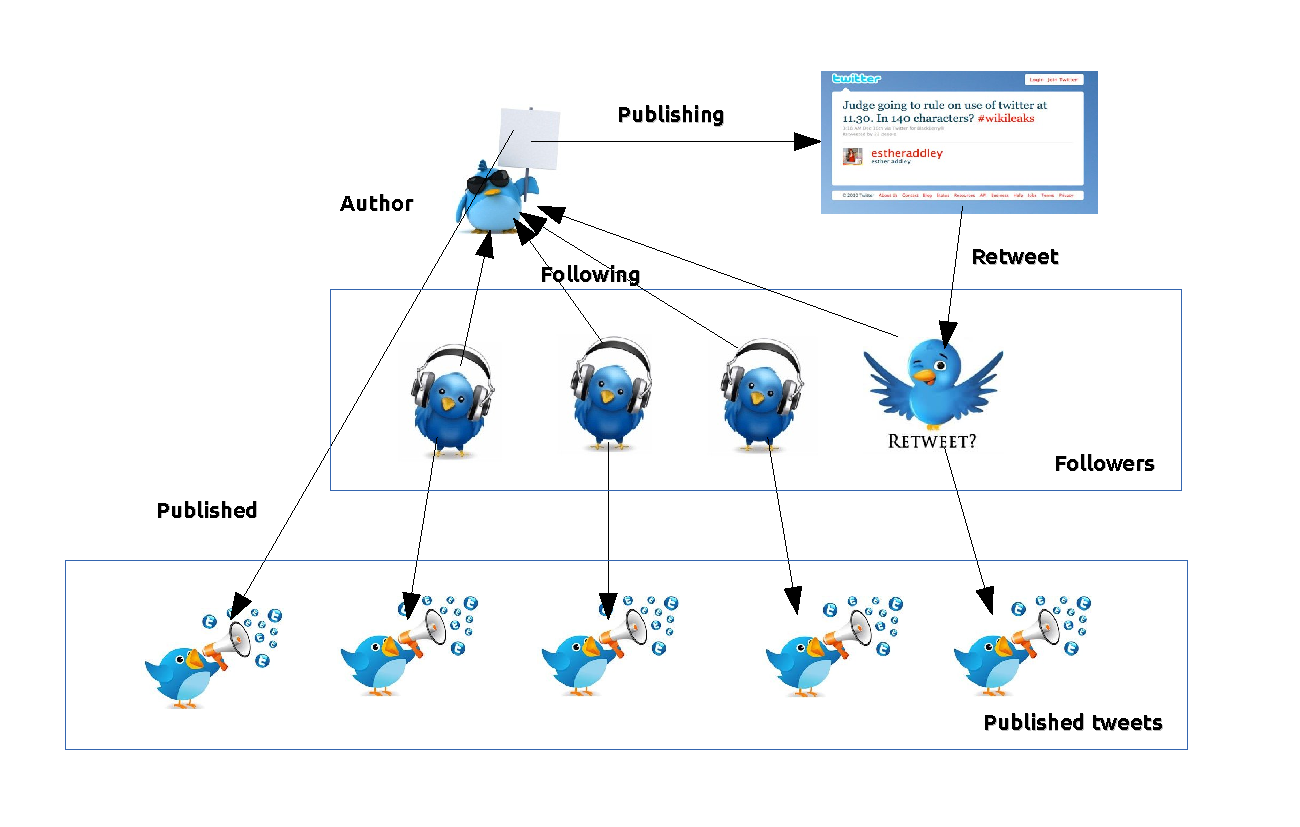
\includegraphics[width=3.5in,height=2.1in]{dataset.pdf}
%\vspace{-4em}
\caption{Illustration of dataset structure.}
\label{fig:graph3}
\end{figure}

There is a local network structure for each tweet of 500 test tweets as figure shows, consisting of its publisher and followers.
We build a local topic space for each local network in which subjective models of users and tweets are built.
As an example, we present subjective models for one of the 500 test tweet, its publisher, and two followers (one retweet the tweet while the other does not) as Figure~\ref{fig:graph4} shows. The right part of each model is topic distribution and the left part is opinion distribution for each topic. It is the 14th topic that the tweet talks about in the local topic space.
%In order to make Figure~\ref{fig:graph4} vividly, we plot top words of the 14th topic ,

Figure~\ref{fig:graph4} plot top words of the 14th topic.

\begin{figure*}[htb]
%\setlength{\belowcaptionskip}{-0.2cm} 
\centering%,bb=0 0 1280 960
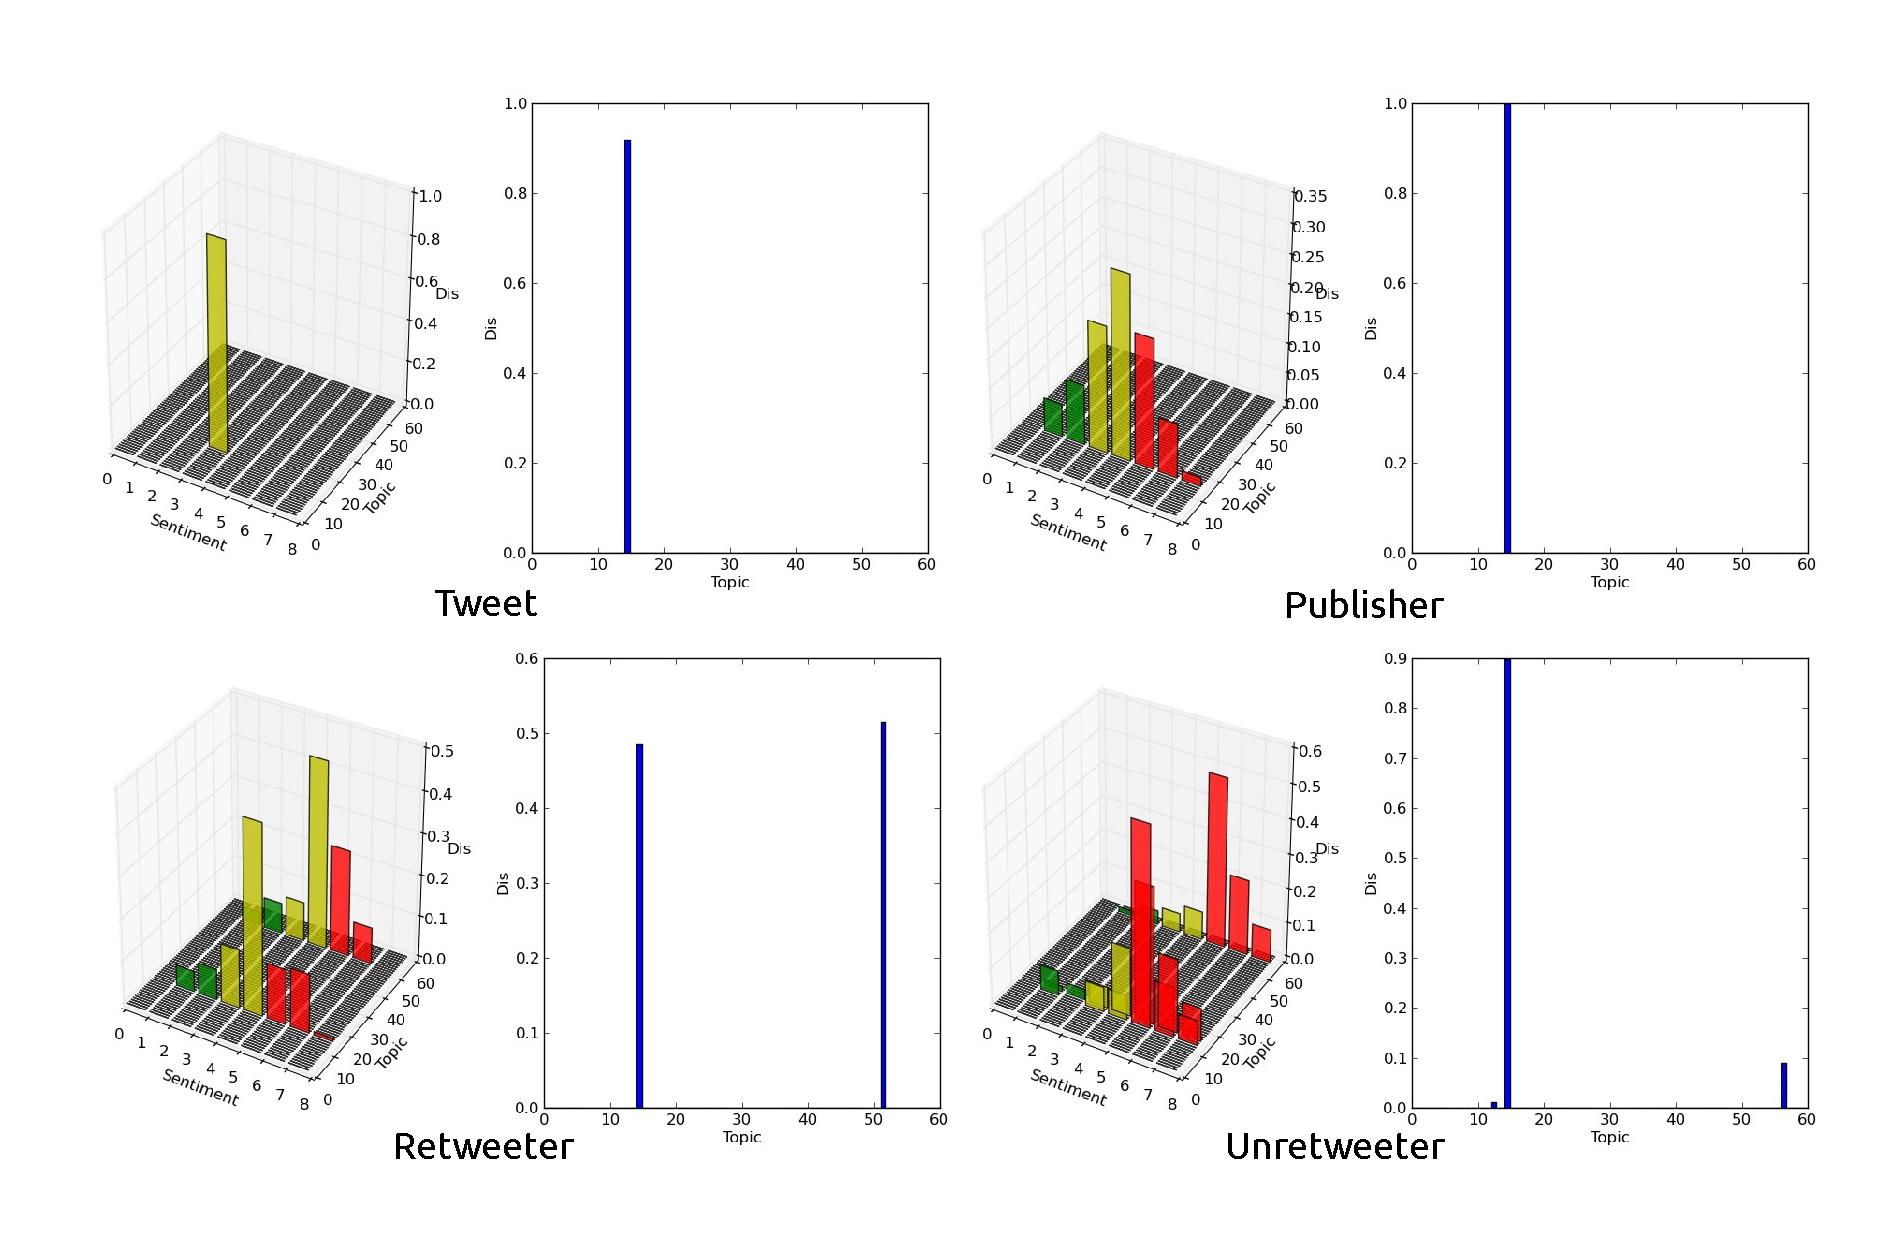
\includegraphics[width=7in,height=4in]{tweets10.pdf}
%\vspace{-4em}
\caption{Subjective model examples.}
\label{fig:graph4}
\end{figure*}

 
Figure~\ref{fig:graph5} shows the tweets of publishers and two followers in a word cloud\footnote{We use TagCrowd (\url{http://tagcrowd.com/}) to produce word cloud.}.


\begin{figure}[htb]
%\setlength{\belowcaptionskip}{-0.2cm} 
\centering
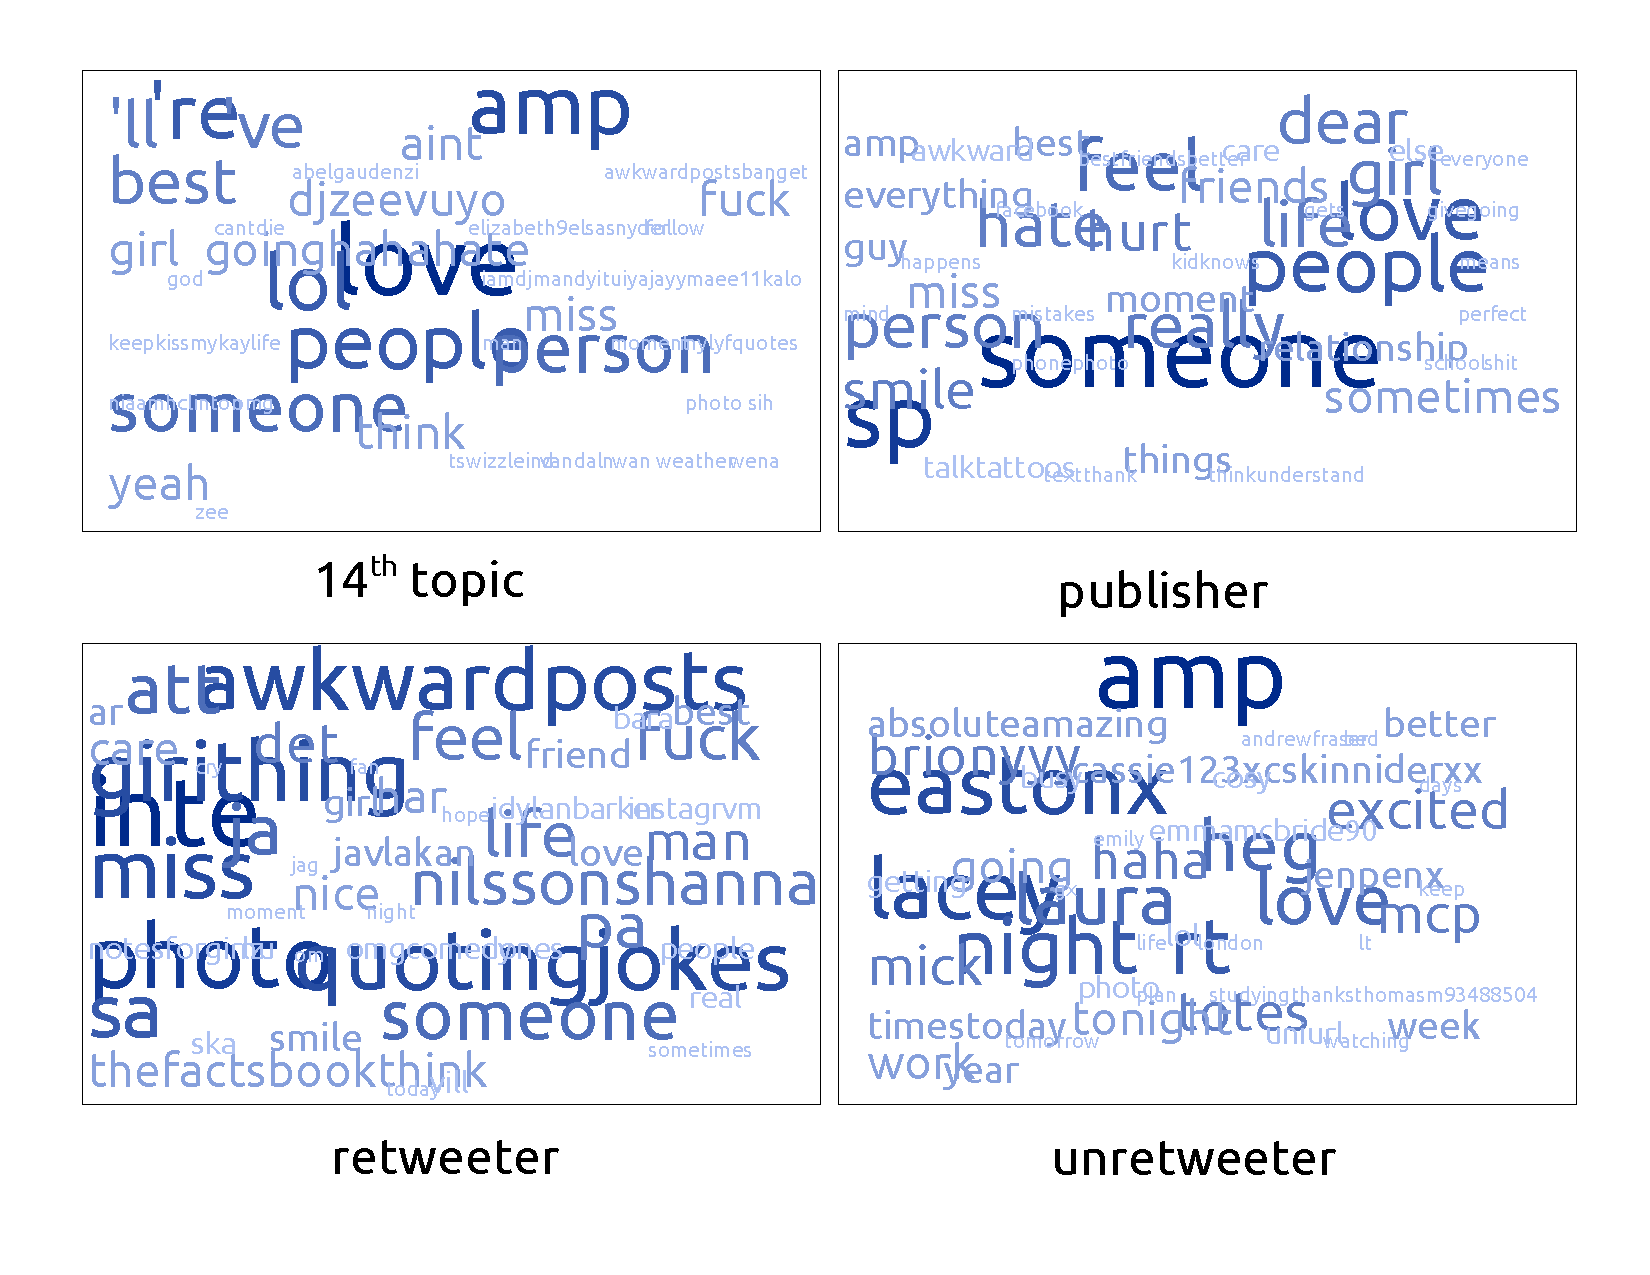
\includegraphics[width=3.5in,height=2.2in]{text_cloud.pdf}
%\vspace{-3em}
\caption{Word cloud of 14th topic, publisher and followers}
\label{fig:graph5}
\end{figure}

%In the example, the test tweet content is:

\textit{Tweet: ``Sometimes the right person for you was there all along. You just didn’t see it because the wrong one was blocking the sight''} is one example.

The topic of this tweet is about ``love between people'' and the opinion is neutral, which is in accordance with the 14th topic word cloud in Figure~\ref{fig:graph5} and subjective model of tweet in Firgure~\ref{fig:graph4}.
The publisher of tweets also talks about ``love between people'', and his opinions are mainly neutral (see Figure~\ref{fig:graph4}).
As for two followers, the ``retweeter'', who retweet the example tweet, has published tweets about two topics (the 14th and 52nd topic) uniformly and his opinions towards the two topics are mainly neutral.
While the other one, who did not retweet the example tweet (we call ``unretweeter''), has also talked about two topics (14th and 56th topic), but he is mainly interested in ``love between people'' topic and has positive opinions.
Although two followers have same interest (the 14th topic), the difference of their opinions towards the topic elicits their different retweet behavior, which verifies our subjective model can help understand the retweet behavior.

\subsection{Influence of Subjective  Model on Retweet}
\label{influence}
In this section we quantitatively investigate the influence of subjective model on retweet behavior with factors derived from it \mo{(rewrite this sentence)}. 
In our formulation of retweet problem we model retweet with subjective model in the form of similarity measurement~\ref{tweetfollower},\ref{pubfollower}.
By setting different value to $ \lambda $, the measurement can be divided into different parts to model different factors that might influence user's retweet behavior, which are:
\begin{itemize*}
\item \textbf{TTF}: \textbf{T}opic similarity between \textbf{T}weet and each \textbf{F}ollower $ \left( \lambda =1  \text{ in measurement~\ref{tweetfollower}} \right) $ 
\item \textbf{OTF}: \textbf{O}pinion similarity between \textbf{T}weet and each \textbf{F}ollower $ \left( \lambda =0 \text{ in measurement~\ref{tweetfollower}} \right) $
\item \textbf{STF}: \textbf{S}ubjective similarity between \textbf{T}weet and each \textbf{F}ollower $ \left( \lambda \in \left( 0,1 \right)   \text{ in measurement~\ref{tweetfollower}} \right) $ 
\item \textbf{TPF}: \textbf{T}opic similarity between \textbf{P}ublisher and each \textbf{F}ollower $ \left( \lambda =1  \text{ in measurement~\ref{pubfollower}}  \right) $ 
\item \textbf{OPF}: \textbf{O}pinion similarity between \textbf{P}ublisher and each \textbf{F}ollower $ \left( \lambda =0 \text{ in measurement~\ref{pubfollower}} \right) $
\item \textbf{SPF}: \textbf{S}ubjective similarity between \textbf{P}ublisher and each \textbf{F}ollower $ \left( \lambda \in \left( 0,1 \right)   \text{ in measurement~\ref{pubfollower}} \right) $
\end{itemize*}

To analyze the influence of different factors on retweeting, we averaged six similarity scores on 5214 followers who retweet the testing tweets and 5214 randomly selected followers who do not retweet separately.  Figure~\ref{fig:graph6} shows the comparing result.

\begin{figure}[htb]
%\setlength{\belowcaptionskip}{-0.2cm} 
\centering
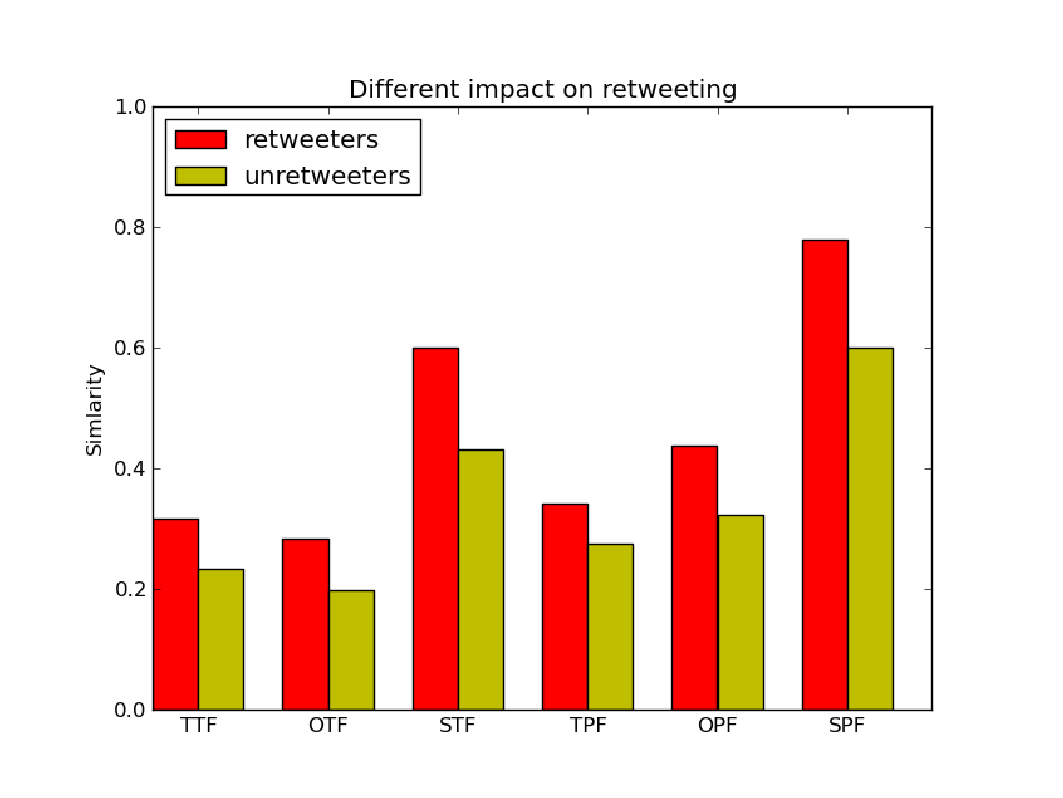
\includegraphics[width=3.5in,height=2.2in]{component.pdf}
%\vspace{-4em}
\caption{Influence of different factors on retweet.}
\label{fig:graph6}
\end{figure}

As the figure demonstrated, on average, the similarities scores of retweeted followers are clearly higher than unretweeted followers for all six factors. It show that our assumption is reasonable\mo{Give the conclusion directly not "our assumption"}. Specifically \mo{not listing},

\begin{itemize*}
\item TTF score shows that a tweet is more likely to be retweeted by followers who find topics it talks about interesting to them, which is consistent with other studies\cite{conf/icwsm/MacskassyM11, conf/wsdm/FengW13};
\item OTF score shows that opinions in a tweet is an important indicator to be retweeted by by followers who hold similar opinions, although other studies\cite{conf/icwsm/PfitznerGS12,2011:NaveedGKC} have shown that sentiment in tweet have impact on retweet, most of them don't consider the opinions of followers and the opinion similarity betweet tweet and its followers;
\item STF score shows the subjective model we put forward is the most distinguishable feature among the six factors with the largest difference between retweeted and unretweeted followers, which proves the importance of subjectivity;
\item TPF score gives another perspective for retweet from the topic similarity between tweet publisher and followers, indicating that followers are more likely to retweet those whose interests are similar, which verifies the homophily principle of retweet relation;
\item OPF score indicates that similar opinions for common topics of interest also influence followers' decision of retweeting anothor user, which may be another proof of homophily of retweet relation.
\item SPF score is interesting in that it implies that subjective similarity between user and follower might cause retweet, and we call this phenomenon ``tight homophily'' because it requires both topic homophily and opinion homophily.
\end{itemize*} 

The six scores used to model the factors that influence retweet could be grouped into two aspects. 
One is consisted of TTF, OTF and STF, which is direct and explicit by modeling the tweet and its followers;
the other is consisted of TPF, OPF and SPF, which is indirect and implicit by modeling the tweet publisher and followers.
The two aspects reflect properly the information sharing and diffusion structure of Twitter at micro-level as illustrated in Figure~\ref{fig:graph3}. \mo{(I do not understand.)}

\subsection{Performance of Retweet Prediction }
\label{performance}
The main purpose of subjective model is to help users find attracting information which could arouse their resonation from the overwhelming information streams\mo{"arouse their resonation" is wrong}. 
In the context of Twitter, retweet is an important signal elicited by such resonation, because users are prone to broadcast their favorite tweets to their followers. 
Thus, the performance of predicting retweet is a suitable measurement for the utility of subjective model. The experiment can be regarded as a simulation of information diffusion process: when a user is browsing message streams he has subscribed for, he might find himself resonate with a tweet and share it with his followers. On the other side, when a new tweet is created, we want to know those followers who will retweet it when reading it.

As Section~\ref{statement} introduced, the retweet problem could be formulated as a tuple $< f, p, c, r_{fpc}> $.
In the prediction experiment we need to estimate the label $ r_{fpc} $ when $ c, p, \text{and } f $ are known. 
There are 5,214 users in our dataset who retweet testing tweets, so we extract 5214 tuples as positive instances with their label $ r_{fpc}=1 $.
The other 40,317 users who do not retweet any testing tweets are also extracted to form negative tuples with label $ r_{fpc}=0 $.
Avoiding unbalance bias of training data, we randomly sample 5,214 negative instances into the final dataset.

\subsubsection{Comparison With Other User Models}
\label{comparison}
Firstly the comparison between our model with other user models (TF-IDF model \cite{Luo:2013RMF}, entity-based model and hashtag-based model \cite{Abel:2011AUM}) in predicting retweet are investigated.
As for our model, the six parts defined above are used for teasing, because they model different factors that influence retweet.
For the comparing models, cosine similarities are calculated between tweets and their followers.
We use the logistic regression classifier of Scikit-learn machine learning package \cite{scikit-learn} for training, with 5-fold cross-validation on our balance dataset. Accuracy is our evaluation metric.

Figure~\ref{fig:graph7} gives the performances of our model and all other models.
\begin{figure}[htb]
%\setlength{\belowcaptionskip}{-0.2cm} 
\centering
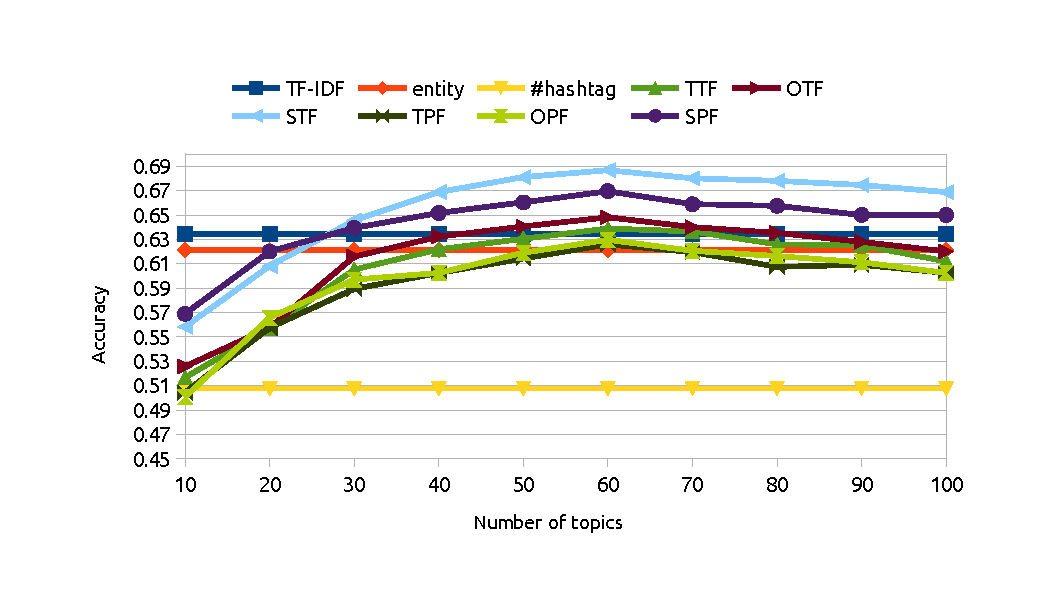
\includegraphics[width=3.5in,height=2.2in]{comparison.pdf}
%\vspace{-4em}
\caption{Comparison of different models.}
\label{fig:graph7}
\end{figure}

The highest accuracy of 68.67\% is the STF (Subjective similarity between Tweet and Followers) model achieved.
The accuracies of TF-IDF model and entity-based model are 63.45\% and 62.12\%, which are very close to our TTF (Topic similarity between Tweet and Followers, 63.88\%) model and OPF (Opinion similarity between Publisher and Followers, 62.96\%) model.
While for hashtag-based model, its accuracy is  50.76\% , which is only little better than random selection (50\%)but not significant. The reason might be that the number of hashtag in our data is not very large. 
The accuracies of the other three model based on our method are OTF (Opinion similarity between Tweet and Followers) model 64.80\%, TPF (Topic similarity between Publisher and Followers) model 62.58\% and SPF (Subjective similarity between Publisher and Followers) model 66.95\%.
The results show that subjective model can better help understand retweet behavior than the other models.

Figure~\ref{fig:graph7} also shows that the influence of topic number of LDA on the predicting accuracy, which arrives its peak when the number is set to 60.

\subsubsection{Retweet Classification Evaluation}
\label{classifiction}
In this section, we feed the six parts of our model as features into a retweeting classification framework to verify the effectiveness of our subjective model. 
We compare the performance of our model with a prediction model of Luo et al. \cite{Luo:2013RMF} which uses four feature families: Retweet History, Follower Status, Follower Active Time and Follower Interests. \mo{You would better introduce these features.}

We use LinearSVM of Scikit-learn package to build a retweet prediction model, leveraging two different features sets. One includes the six features derived from subjective model (marked as ``SM6''). The other is Luo et al. \cite{Luo:2013RMF}(marked as ``LUO'') feature set in which they use ``bag-of-words'' to model the followers interest.  We use the same dataset as introduced in Section~\ref{comparison} with 5-fold cross-validation, and accuracy as evolution metric.
In addition, we set a baseline (marked as ``RB''), in which followers who have retweeted the publisher's previous tweets before are predicted as retweeters for current tweet. 

The result is listed in Table~\ref{table2}.
\begin{table}
\centering
\caption{Prediction Accuracy of Different Models. Significant improvement over baseline with star($ \ast $) and LUO' model with dagger($ \ddagger $) (p$ < $0.05).}
\label{table2}
\begin{tabular}{|l|l|}
\hline
Feature Set & Accuracy(\%) \\
\hline
RB & 60.85  \\
LUO & 68.76 $ \ast  $\\
SM6 & 69.12  $ \ast $ \\
LUO($ \ominus $)+TTF & 69.20  $ \ast $ \\
LUO($ \ominus $)+TPF & 71.04  $ \ast \quad \ddagger $ \\
LUO($ \ominus $)+OTF & 71.88  $ \ast \quad \ddagger $ \\
LUO($ \ominus $)+OPF & 70.27  $ \ast $ \\
LUO($ \ominus $)+STF & 72.86  $ \ast \quad \ddagger $ \\
LUO($ \ominus $)+SPF & 72.05  $ \ast \quad \ddagger $ \\
LUO($ \ominus $)+All & 72.93  $ \ast \quad \ddagger $ \\
\hline
\end{tabular}
\end{table}
The accuracy of baseline is 60.85\% Both prediction model based on sets of features (LUO and our SM6) outperform the baseline significantly. 
But the prediction model based on our feature set shows no significant improvement over the model based on LUO feature set. The reason might be that our model only tries to reflect the retweet motivation of users based on content, whereas other important factors associated with retweet are not considered, such as network context and reading habit of the user. 
As denoted by ``LUO($ \ominus $)+'' in the table, we combine the two sets of features by replacing the Follower Interests features of LUO model with our six features one by one. 
The accuracies are all improved. It shoes that our model is of great importance for retweet prediction models. 
Notice that, the most significant improvement (LUO($ \ominus $)+STF, 72.86\% versus 68.76\%) is the subjective similarity features between tweet and followers, which verifies our assumption that resonation between tweet and the followers elicits retweet behavior\mo{(wrong sentence)}.
Besides, the improvement by adding subjective similarity features between publisher and followers (LUO($ \ominus $)+SPF, 72.05\% versus 68.76\%) is also obvious in that the resonation between publisher and follower indicates the tight homophily between them.
Finally, the last row of table is the complete combination of two sets of features (LUO($ \ominus $)+All) by adding all six features into LUO feature set. The performance shows no significant improvement over adding STF feature only \mo{(reason?)}.
\section{Conclusion}
In this paper, we propose subjective model to analyze user retweeting behavior on Twitter. We assume that retweeting behavior should be elicited by the subjective resonation between the tweet and its followers. 
We define subjective model formally as combination of topic distribution and opinion distribution, and we concrete subjective model leveraging statistical topic model and sentiment analysis techniques.
We demonstrate the effectiveness of our proposed model with retweeting analysis problem and show that this model is able to reach more comprehensive understanding of retweeting. 

Our future work mainly lies in two directions.
Firstly, our subjective model is established in a simple way. It is an interesting direction to establish it under the framework of generative topic-sentiment model, which has been applied in reviews and citation network.
Secondly, we will apply subjective model to other social media analysis task such as connection prediction and friend recommendation.
\bibliographystyle{abbrv}
\bibliography{resonate_tweet}
\end{document}
